% SYNC injection through the SN74HC240 ground pin, and the edge-current loop it creates.
% Build: lualatex sync-ground-bounce.tex && pdftoppm -png -r 300 -singlefile sync-ground-bounce.pdf sync-ground-bounce
\documentclass[border=8pt]{standalone}
\usepackage[siunitx, american]{circuitikz}
\usepackage{fontspec}
\setmainfont{TeX Gyre Heros}
\usepackage{sansmath}
\sansmath
\sisetup{mode=text}

\definecolor{cur}{HTML}{D4B400}  % matches scope CH1 yellow
\definecolor{plane}{HTML}{9AA7B0}

\begin{document}
\ctikzset{bipoles/thickness=1}
\begin{circuitikz}[
    font=\small,
    line width=1pt,
    curw/.style={draw=cur, line width=1.2pt, -{Latex[length=2.2mm]}},
    retw/.style={draw=cur, line width=1pt, dashed, -{Latex[length=2.2mm]}},
    chip/.style={draw, line width=1pt, fill=white, minimum width=2.8cm, minimum height=1.4cm, align=center},
  ]

  % Ground plane
  \fill[plane!40] (-1.6,-0.12) rectangle (14.4,0.12);
  \node[text=plane!80!black, font=\scriptsize\bfseries, anchor=north west] at (-1.6,-0.15) {GND PLANE};

  % Oscillators and SYNC filter on one row: +3.3 V into VCC, GND pin 10 is the SYNC net
  \node[chip] (osc) at (4,1.8) {Oscillators A--H};
  \node[chip] (filt) at (10.2,1.8) {Filter};
  \draw (0,1.8) node[left] {+\SI{3.3}{V}} -- (osc.west);
  \fill (0,1.8) circle (1.5pt);
  \draw (0,1.8) to[C] (0,0);
  \node[align=right, anchor=east] at (-0.4,0.8) {$C_5$\\\SI{100}{nF}};
  \node[font=\scriptsize\bfseries, anchor=south east] at (osc.west) {VCC};
  \draw (osc.east) -- (filt.west);
  \node[font=\scriptsize\bfseries, anchor=south west] at (osc.east) {GND (10)};
  \node[font=\small\bfseries, anchor=south] at (8.1,1.85) {SYNC};
  \draw (7,1.8) -- (7,2.25);
  \draw[fill=white] (7,2.4) circle (0.15) node[right=1pt, font=\scriptsize] {J5};
  \draw (filt.south) -- (10.2,0);

  % SYNC input (J8 BNC): voltage source from the filter to the plane
  \draw (filt.east) -- (13,1.8) -- (13,1.25);
  \draw (13,0.55) -- (13,0);
  \draw[fill=white] (13,0.9) circle (0.35);
  \draw[-{Triangle[length=2mm, width=2mm]}] (13,0.65) -- (13,1.15);
  \node[font=\scriptsize, align=left, anchor=west] at (13.4,0.9) {\textbf{SYNC}\\J8 BNC};

  % Edge-current loop: C5 -> VCC -> oscillators -> GND pin -> SYNC -> filter -> plane -> C5
  \draw[curw] (0.3,1.15) -- (0.3,1.5) -- (2.6,1.5);
  \draw[curw] (5.4,1.5) -- (8.8,1.5);
  \draw[retw] (9.9,1.1) -- (9.9,0.35) -- (0.3,0.35) -- (0.3,0.65);
  \node[text=cur, font=\small\bfseries, anchor=north] at (10.2,-0.2) {$\approx\SI{50}{\ohm}$ at \SI{2}{MHz}};

  % Measured J5 vs GND, no SYNC applied: CH1 (yellow, 100 mV/div) J5, CH2 (purple, 1 V/div) OSC_A_L
  \node[inner sep=0, draw=plane, line width=0.4pt, anchor=center] (scope) at (10.4,4.0)
    {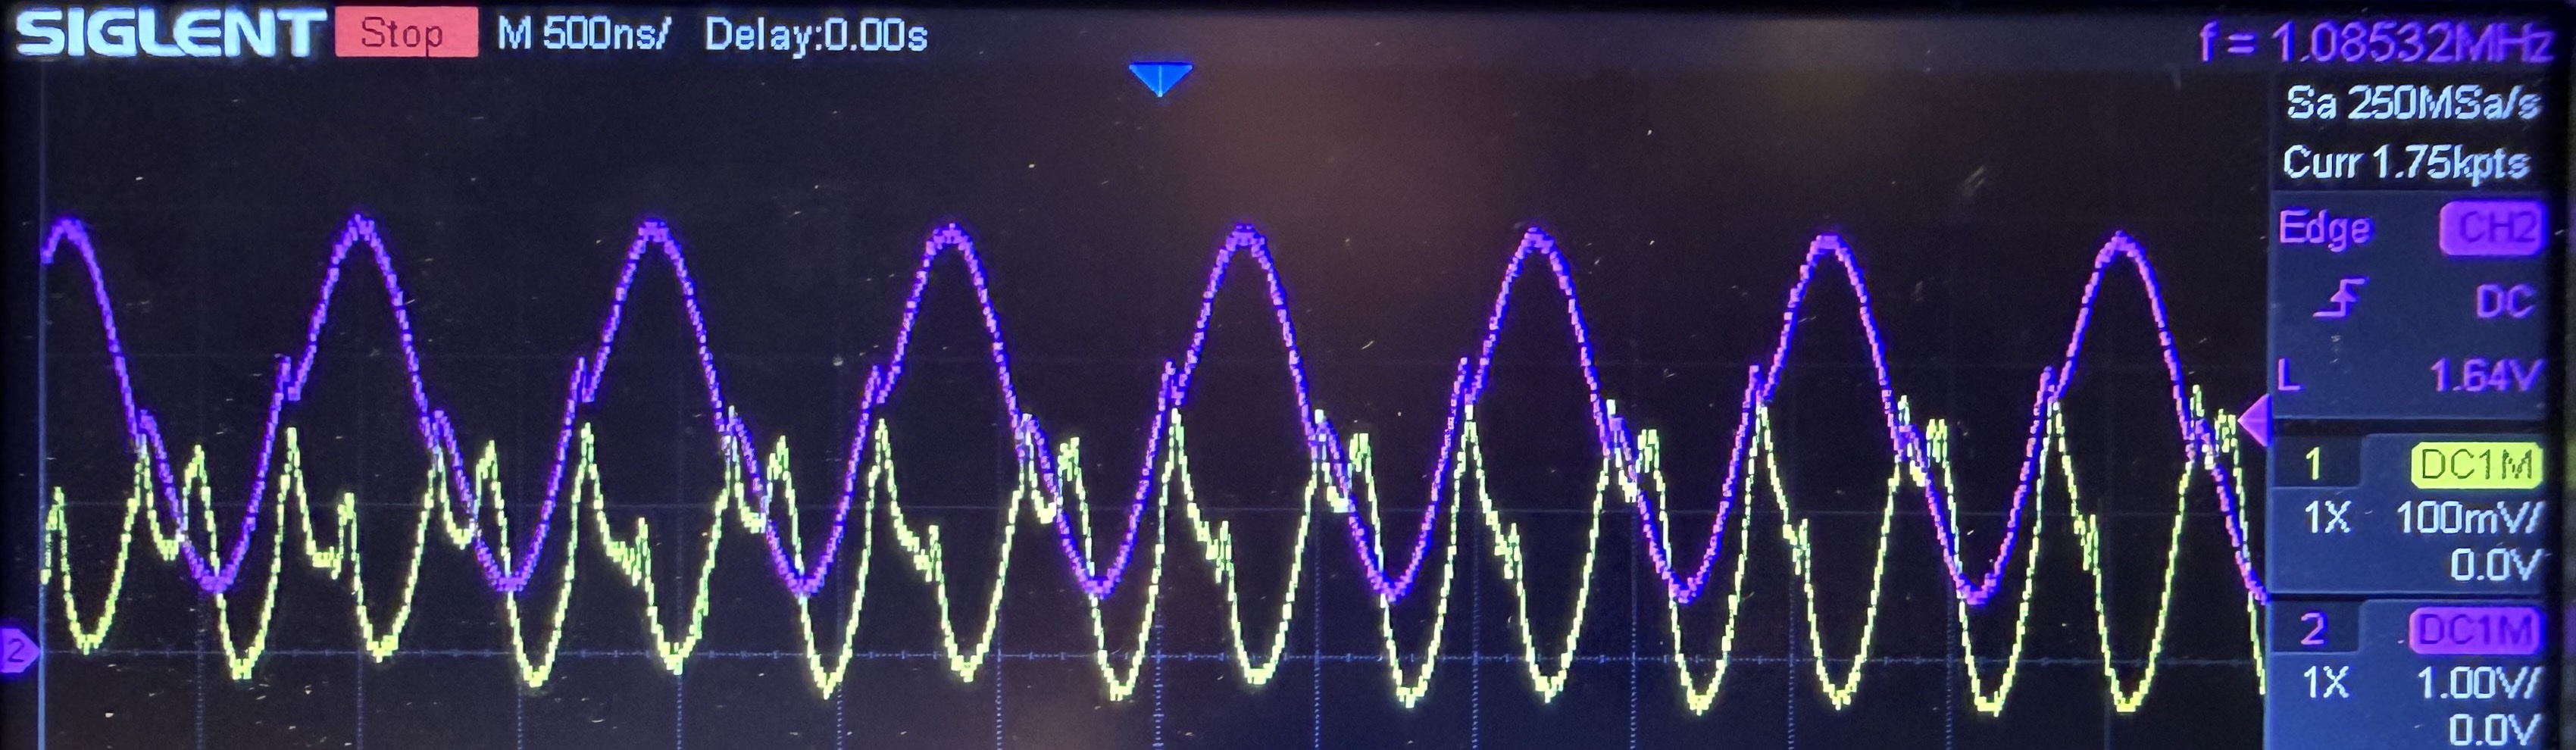
\includegraphics[width=4.8cm]{sync-ground-bounce-scope.jpg}};
  \node[font=\scriptsize, text=cur, anchor=north, align=center] at (scope.south)
    {J5, no SYNC: $\approx\SI{300}{mV_{pp}}$ at \SI{2}{MHz} $= 2f_\mathrm{osc}$\\(CH2: OSC\_A\_L)};
\end{circuitikz}
\end{document}
